\documentclass[11pt]{article}
\usepackage[T1]{fontenc}
\usepackage{lmodern,microtype}
\usepackage[margin=1in]{geometry}
\usepackage{amsmath,amssymb,amsthm,mathtools}
\usepackage{booktabs,array,longtable,enumitem,graphicx,xcolor}
\usepackage[hidelinks]{hyperref}
\hypersetup{pdftitle={Exactly Five Platonic Solids},
 pdfauthor={Prepared for Vladimir Reshetnikov},
 pdfsubject={A finite constructive classification in intuitionistic primitive recursive arithmetic},
 pdfkeywords={Platonic solids, iPRA, constructive geometry, Lean}}
\usepackage{fancyhdr}
\setlength{\headheight}{14pt}
\pagestyle{fancy}\fancyhf{}
\fancyhead[L]{\small Exactly five Platonic solids}
\fancyhead[R]{\small Constructive arithmetic}
\fancyfoot[C]{\thepage}
\setlength{\parskip}{4pt}
\setlength{\parindent}{0pt}
\setlist{itemsep=3pt,topsep=5pt}
\newtheorem{theorem}{Theorem}[section]
\newtheorem{lemma}[theorem]{Lemma}
\newtheorem{proposition}[theorem]{Proposition}
\newtheorem{corollary}[theorem]{Corollary}
\theoremstyle{definition}
\newtheorem{definition}[theorem]{Definition}
\newtheorem{remark}[theorem]{Remark}
\newcommand{\ipra}{\mathsf{iPRA}}
\newcommand{\N}{\mathbb N}
\newcommand{\Z}{\mathbb Z}
\newcommand{\Q}{\mathbb Q}
\newcommand{\R}{\mathbb R}
\newcommand{\K}{\mathbb K}
\newcommand{\sgn}{\operatorname{sgn}}
\newcommand{\conv}{\operatorname{conv}}
\newcommand{\cyc}{\operatorname{cyc}}
\newcommand{\Valid}{\operatorname{Valid}}
\newcommand{\Class}{\operatorname{Class}}
\newcommand{\Witness}{\operatorname{Witness}}
\newcommand{\Similar}{\operatorname{Similar}}
\newcommand{\Model}{\operatorname{Model}}
\newcommand{\code}[1]{\texttt{#1}}
\title{\textbf{Exactly Five Platonic Solids}\\[6pt]
\large A finite constructive classification in\\intuitionistic primitive recursive arithmetic}
\author{Prepared for Vladimir Reshetnikov}
\date{November 15, 2026}
\begin{document}
\maketitle
\begin{abstract}
There are exactly five similarity classes of convex regular polyhedra:
the tetrahedron, cube, octahedron, dodecahedron, and icosahedron.
We give a human-readable proof with an explicit interpretation in
intuitionistic primitive recursive arithmetic. Inputs are finite polyhedra
with exactly represented constructible coordinates, congruent regular
polygonal facets, and a common vertex valence. The proof establishes
Euler's identity by finite counting, classifies the five numerical and
combinatorial cases, proves the necessary finite rigidity result, and
constructs all five examples in $\Q(\sqrt5)$. Every search has a finite
bound; no real-number completeness, choice principle, or undecidable
real comparison is used. A primitive recursive classifier returns a
similarity certificate. The archive includes exact executable certificates
and a Lean roadmap tied to ProveIt's existing embedded $\ipra$ syntax.
The supplied Lean source is an \emph{uncompiled arithmetic prototype};
the complete geometric derivation has not been kernel-checked.
\end{abstract}
\newpage
\tableofcontents
\newpage
\section{What is being counted, and what is proved internally}

The number is \textbf{five}, where position, orientation, and positive scale
are disregarded. There are of course infinitely many placed or scaled
tetrahedra. Reflections are allowed in the equivalence relation.

\begin{definition}[Geometric input]
A Platonic polyhedron is a bounded, full-dimensional convex polyhedron
whose maximal two-dimensional faces are congruent convex regular polygons,
and for which the same number of faces meets at every vertex. If each
face has $p$ sides and each vertex has valence $q$, its type is $(p,q)$.
Faces are maximal facets: an artificial subdivision does not create new
faces for this definition.
\end{definition}

We retain this usual local definition. In particular we do not assume
flag transitivity, or assume that the type already determines the shape.
Those shortcuts would hide part of the classification problem.

\subsection{The finite coordinate domain}

First-order arithmetic has natural numbers as its objects. A sentence
about all unspecified set-theoretic real polyhedra is not literally a
sentence of $\ipra$. Our internal objects therefore have the following
explicit representation.

A scalar is a finite expression obtained from rational numbers by
addition, subtraction, multiplication, division by a nonzero scalar,
and the nonnegative square root of a nonnegative scalar. Equivalently,
place a finite collection of such expressions in a common tower
\[
 \Q=K_0\subseteq K_1\subseteq\cdots\subseteq K_n,
 \qquad K_j=K_{j-1}(s_j),\quad s_j^2=r_j\geq0.
\]
The extensions need not have degree two: $r_j$ may be zero or a square
already in $K_{j-1}$. This redundancy must be respected by equality.
All points of the input use one common finite tower. New auxiliary square
roots are appended to it. This is the field of real constructible scalars,
presented by finite codes; it is not a representation of arbitrary
computable real numbers.

A polyhedron code lists distinct vertices, its facet cycles, and their
incidences. Face cycles have distinct vertices, and duplicate facet
vertex sets are forbidden. The validator checks the following finite conditions:
\begin{enumerate}
\item Four listed vertices are affinely independent. Each listed vertex
is an extreme point, and every facet is a convex planar cycle.
\item For each facet an oriented cross-product normal gives a supporting
plane. Its equality set among the vertices is exactly the facet's vertex
set; all other vertices lie strictly on the inner side.
\item All facets occur. This is checked by examining every noncollinear
vertex triple: whenever its plane is supporting, its full equality set
must be one of the listed facets.
\item Edges are the consecutive vertex pairs on facet boundaries.
Every edge belongs to two facets; each vertex link is one cyclic list;
the face adjacency graph is connected. These are also consequences of
the convex hull description, but checking them makes the data interface
particularly transparent.
\item The facets have common size $p\geq3$, are regular and congruent,
and the vertex links have common length $q\geq3$.
\end{enumerate}
Extreme-point status can be checked without linear programming: the
normals of the incident supporting planes must span three dimensions.
For a supporting-plane intersection this is equivalent to a zero-dimensional
face. Completeness of the facet list follows from the elementary fact
that every facet of a full-dimensional finite hull contains three
affinely independent vertices. Conversely the equality set of every
supporting noncollinear triple is exactly the vertex set of a facet,
so the test adds no extraneous facets.

Regularity has a convenient exact test. Center the ordered vertices
$x_0,\ldots,x_{p-1}$ of a face at their average. Require its Gram matrix
to be invariant under $(i,j)\mapsto(i+1,j+1)$ modulo $p$. Cyclic shift
then extends to an isometry of the face plane. Since it preserves the
convex cyclic order, it is a rotation carrying each vertex to its
successor. This is exactly a convex regular polygon. Equality of the
corresponding face Gram matrices tests congruence. Thus no trigonometric
function is needed even to state regularity.

\begin{theorem}[Internal finite classification]\label{thm:main}
There are fixed primitive recursive functions $\Valid$, $\Class$, $\Witness$,
and $\Similar$, and five fixed model codes $\Model(0),\ldots,\Model(4)$,
for which $\ipra$ proves
\begin{align*}
 \Valid(c)=1\ \Longrightarrow\ &\Class(c)<5\ \wedge\\[-4pt]
 &\Similar(c,\Model(\Class(c)),\Witness(c))=1.
\end{align*}
It also proves that the five model codes are valid and pairwise
non-similar. The similarity certificate contains a vertex bijection
and an affine map $x\mapsto Ax+b$ satisfying
$A^{\mathsf T}A=\lambda I$ for a positive scalar $\lambda$.
\end{theorem}

This is a theorem with a constructive witness, rather than an appeal to
a quotient whose number of elements is assumed to exist. The proof of
the theorem is the mathematical argument below, together with its
explicit primitive recursive implementation described in
Section~\ref{sec:internal}. A machine-checked derivation in the embedded
syntax remains a formalization task.

\begin{remark}[Relation to the ordinary theorem]
All five representatives have coordinates in $\Q(\sqrt5)$. The same
geometric proof, interpreted externally over ordinary $\R$, gives the
usual unrestricted classical classification. Thus the finite theorem
captures all five shapes. It does not assert that arbitrary real-number
names can be compared or normalized by a primitive recursive program.
\end{remark}

\subsection{Exact order and why the scalar algorithms are primitive recursive}

The only potentially delicate computational ingredient is exact sign.
Here are explicit algorithms, including redundant tower stages.
At one stage write $x=a+bs$, where $s^2=r\geq0$ and all of $a,b,r$
belong to the preceding stage. If $r=0$, return the sign of $a$.
Otherwise handle $a=0$ or $b=0$ directly. If $a,b$ have the same sign,
that is the sign of $x$. If their signs are opposite, then
\begin{equation}\label{eq:towersign}
 \sgn(a+b\sqrt r)=\sgn(a)\,\sgn(a^2-b^2r).
\end{equation}
Indeed, when $a>0>b$, comparison with zero is precisely the comparison
of the two positive quantities $a$ and $(-b)\sqrt r$; squaring preserves
that comparison. The other case follows by negation. Every comparison
on the right is in a strictly shorter tower.

Addition and multiplication are
\[
 (a,b)+(c,d)=(a+c,b+d),\qquad
 (a,b)(c,d)=(ac+bd r,ad+bc).
\]
For inversion put $N=a^2-b^2r$. If $N\ne0$, use
\[
 (a+bs)^{-1}=(a-bs)/N.
\]
If $N=0$ and $r>0$, then $a$ and $bs$ have equal absolute value.
If $a=0$ or the signs of $a,b$ are opposite, the element is zero;
otherwise $a+bs=2a\ne0$, and its inverse is $1/(2a)$ in the preceding
stage. For $r=0$ invert $a$ directly. Define the inverse of zero to be
zero as a totalization, and reject a division by zero when validating
an expression. Equality is sign zero, \emph{not} coefficientwise equality
at a possibly redundant stage. The following lemma proves the required
ordered-field laws; quotient notation is only shorthand for the
decidable equality relation on codes.

\begin{lemma}[One ordered quadratic stage]\label{lem:orderedstage}
Let $K$ be a decidably ordered field and $r\geq0$ in $K$. On formal
pairs $a+bs$ use the displayed addition, multiplication, and sign
algorithms, with $s^2=r$. Define $x\sim y$ when $\sgn(x-y)=0$.
Then $\sim$ is a ring congruence, sign is well-defined modulo $\sim$,
and the represented structure is an ordered field with $s\geq0$
and $s^2=r$.
\end{lemma}
\begin{proof}
If $r=0$, operations and sign reduce to evaluation $a+bs\mapsto a$.
Assume $r>0$. First, whenever $t>0$ in $K$ satisfies $t^2=r$, the
prescribed sign of every $c+ds$ equals $\sgn_K(c+dt)$. In the
opposite-sign case this is precisely comparison by squaring the
two nonnegative quantities; all other cases are immediate.
Evaluation at such a $t$ respects addition and multiplication.

This observation handles redundant representations without a test
for whether $r$ has a square root in $K$. If $\sgn(a+bs)=0$ but
$(a,b)\ne(0,0)$, the sign cases give $b\ne0$ and the explicit root
$t=-a/b>0$, $t^2=r$. Whenever an equality premise has a nontrivial
zero difference, this $t$ reduces sign invariance, transitivity,
and compatibility with operations to the corresponding facts in $K$.
If every zero difference in the premises is the literal coefficient-zero
pair, the facts hold coefficientwise. Hence $\sim$ is an equivalence
and ring congruence, and sign is invariant under $\sim$.
The ring identities themselves follow by expanding coefficients
using $s^2=r$. Directly from the sign rule,
$\sgn(-x)=-\sgn(x)$, and multiplication by a positive scalar from
$K$ preserves sign.

We explicitly prove the two order-closure properties. Define predicates
solely in the base field:
\[
 L(u)\ \Longleftrightarrow\ u<0\ \text{or}\ (u\geq0\ \text{and}\ u^2<r),
 \qquad
 U(u)\ \Longleftrightarrow\ u>0\ \text{and}\ u^2>r.
\]
$L$ is downward closed, $U$ is upward closed, and $L(l),U(u)$ imply
$l<u$, by monotonicity of squaring on nonnegative elements.
Every positive pair has exactly one of these three forms: a positive
scalar; $b(s-l)$ with $b>0$ and $L(l)$; or $e(u-s)$ with $e>0$ and
$U(u)$. This rewrites the sign rule according to the sign of the
$s$ coefficient.

Two lower forms add to a lower form whose threshold is the positive
weighted average of their thresholds. This is no greater than their
maximum, so $L$ holds. Two upper forms use the corresponding minimum
and $U$. Adding a positive scalar lowers a lower threshold or raises
an upper threshold. For the remaining case add
$b(s-l)+e(u-s)$, where $l<u$. If $b=e$ the sum is $b(u-l)>0$.
If $b>e$, it is $(b-e)(s-l')$, with
\[
 l'=l-\frac{e(u-l)}{b-e}<l,
\]
so $L(l')$ holds. If $b<e$, it is $(e-b)(u'-s)$, with
\[
 u'=u+\frac{b(u-l)}{e-b}>u,
\]
so $U(u')$ holds. Thus the sum of two positive pairs is positive,
without presupposing an order on the extension.

For multiplication put $N(a,b)=a^2-b^2r$. Expansion gives
$N(xy)=N(x)N(y)$. If a positive $x=a+bs$ has $N(x)=0$, its
coefficients $a,b$ are both positive. The explicit root $t=a/b$
and the evaluation observation reduce positivity of its product
with any positive pair to positivity in $K$. The same applies to $y$.
Otherwise, positivity and $N(x)>0$ imply $a>0$, $a^2>b^2r$;
positivity and $N(x)<0$ imply $b>0$, $b^2r>a^2$.
Write $y=c+ds$ and $xy=A+Bs$, where
$A=ac+bdr$, $B=ad+bc$. The four possibilities are
\[
\begin{array}{ccl}
 N(x)>0,\ N(y)>0 &: & ac>|bd|r,\quad A>0,\quad N(xy)>0;\\
 N(x)<0,\ N(y)<0 &: & bdr>|ac|,\quad A>0,\quad N(xy)>0;\\
 N(x)>0,\ N(y)<0 &: & ad>|bc|,\quad B>0,\quad N(xy)<0;\\
 N(x)<0,\ N(y)>0 &: & bc>|ad|,\quad B>0,\quad N(xy)<0.
\end{array}
\]
Each first inequality follows by squaring its positive left side
and multiplying the preceding nonnegative inequalities, cancelling
$r>0$ in the mixed cases. For example, in the third case
\[
 (a^2-b^2r)d^2r+b^2r(d^2r-c^2)>0
\]
is exactly $r((ad)^2-(bc)^2)>0$. The first summand is strictly
positive, since $d>0$. The sign algorithm therefore declares the
product positive in all four cases.

Sign trichotomy, negation, congruence, and the two closure results
give a translation-invariant linear order compatible with
multiplication. For inverses, when $N(x)\ne0$ the conjugate formula
multiplies to one coefficientwise. When $N(x)=0$ but $x$ is nonzero
modulo $\sim$, $a,b$ have the same nonzero sign; $t=a/b>0$ satisfies
$t^2=r$, evaluation sends $x$ to $2a$, and the scalar $1/(2a)$
multiplies with $x$ to one modulo $\sim$. This proves the field
assertion. The element $(0,1)$ is positive and squares to $(r,0)$.

This proof supplies a fixed finite family of base-field templates:
the equivalence and congruence laws, commutative-ring identities,
sign trichotomy and negation, closure of positivity under addition
and multiplication, and the nonzero-inverse identity. Every division
has an explicit nonzero premise; every split is a decidable scalar
comparison. These are the templates used in the bounded law-table
induction below.
\end{proof}

For clarity, a size bound accompanies this recursive description.
Store a level-$n$ element as a dense binary tree of rational coefficient
pairs, and let $H\geq1$ bound the binary lengths of all input and tower
radicand numerators and denominators. Addition, multiplication, sign,
and the displayed inversion algorithm make at most sixteen calls to
strictly lower-level routines at any node. Scalar multiplication here
is a lower-level multiplication, not an additional same-level call.
There are therefore fewer than $16^{n+1}$ nodes in an operation's
expanded call tree. A deliberately larger bound, allowing validation
and bookkeeping, is
\[
 L(n)=2^{16(n+1)}.
\]
Unnormalized rational operations change a coefficient length bound $B$
to at most $2B+1$. Consequently
\begin{equation}\label{eq:bitbound}
 B(n,H)=(H+2)\,2^{L(n)}
\end{equation}
bounds the intermediate coefficient lengths. Standard binary coding of
the finite coefficient arrays and an explicit stack now implement the
algorithms by bounded loops. Long integer arithmetic also has bounded
loops. Both bounds are primitive recursive. Finite sequences of these
operations use primitive recursion on their length, updating the bound
at each step. Appending a root increases the tower depth by one.

These are bounds for computations of the basic operations. A sequence
of $K$ operations is bounded by replacing $L(n)$ with $K L(n)$, or by
iterating the one-operation bound. The ordered-field laws for
represented equality require the bounded law-table construction in
Section~\ref{sec:internal}: fix the final height and coefficient budget,
propagate larger budgets to shorter prefixes, and induct on equations
asserting correctness of the finite tables. Thus no induction on an
unbounded universally quantified field-law assertion is required.
Both the size bounds and the correctness argument matter; mere
termination of an unspecified symbolic procedure would not suffice.

\subsection{The arithmetic theory being used}

We use intuitionistic first-order logic with equality, symbols for
primitive recursive functions, their defining equations, the successor
axioms, and induction for quantifier-free formulas. This is the
presentation in ProveIt's \code{ConciseIPRA/PR.lean}~\cite{proveit}.
We do not add induction for arbitrary formulas.

A bounded assertion over a coded list is represented by a primitive
recursive Boolean fold. An induction invariant is an equation saying
that this fold equals one, together with equations for the accumulated
counts and witnesses. Thus bounded universal checks do not require
stronger induction. All case splits below are on natural-number or exact
scalar comparisons whose decisions were just constructed. We use neither
excluded middle for arbitrary propositions, Markov's principle, choice,
nor a universal evaluator for arbitrary primitive recursive programs.

\section{Finite convex geometry and Euler's identity}\label{sec:euler}

We first record the finite geometric facts used in the proof. A line
intersects a convex polygon in an interval: substitute its affine
parameter into the finitely many half-plane inequalities and take the
largest lower bound and the smallest upper bound. A convex polygon is
triangulated by the diagonals from any one vertex. A point in the polygon
is located in one of those triangles by finitely many determinant signs,
and its barycentric coefficients are obtained by a $2\times2$ inverse.
These statements use exact arithmetic and finite minimum selection.

At a vertex $v$ of a three-dimensional convex polyhedron, intersect its
tangent cone with a plane strictly separating $v$ from the other
vertices. Such a plane is explicit: add the inward deficits of the
incident supporting planes, which vanish simultaneously only at $v$,
and choose a positive level smaller than all the finitely many values
at other vertices. The section is a convex polygon. Its vertices are
the intersections with the edge rays, in their cyclic order. A direction
from $v$ into the polyhedron is a nonnegative combination of edge rays:
intersect it with the section and use the preceding polygon triangulation.
Inserting diagonals in facets merely subdivides edges of this vertex
figure. These observations prove the local cyclic-link properties used
below directly from the finite supporting inequalities.

\begin{lemma}[Generic finite height]\label{lem:height}
For $V$ distinct exactly represented points in three dimensions one can
construct a linear functional taking distinct values on all the points
by trying at most $2\binom V2+1$ integer candidates.
\end{lemma}
\begin{proof}
Try $h_t(x,y,z)=x+ty+t^2z$ for integers
$0\leq t\leq2\binom V2$. For any distinct pair of points, equality of
their heights is a nonzero polynomial equation of degree at most two
in $t$. Such a polynomial has at most two distinct roots, by division
by linear factors. There are at most $2\binom V2$ forbidden values.
Testing the displayed list therefore returns a valid candidate.
This is the finite pigeonhole argument on decidable lists.
\end{proof}

\begin{lemma}[Euler by lower-neighbor counting]\label{lem:euler}
For a finite full-dimensional convex polyhedron,
\[
 V+F=E+2.
\]
\end{lemma}
\begin{proof}
Triangulate each facet by a fan without adding vertices. Each diagonal
adds one edge and one face, so the value of $V-E+F$ is unchanged.
Choose the generic height of Lemma~\ref{lem:height}. Assign every edge
and every triangle to its highest vertex. At a vertex $v$ let $d_v$
count its lower neighbors and $t_v$ its incident triangles whose other
two vertices are lower. Its contribution to $V-E+F$ is
\[
 1-d_v+t_v.
\]
In the convex vertex figure, being lower is an affine half-plane
condition. The lower neighbors therefore form a consecutive block
in the cyclic order, unless all or none of them are lower. For a
nonempty proper block, $t_v=d_v-1$, and the contribution is zero.
If all neighbors are lower, the edge-ray combination property proves
that $v$ is the unique global maximum; its full cyclic link gives
$t_v=d_v$, so its contribution is one. If none is lower, the same
argument makes $v$ the unique global minimum; its contribution is one.
There are no other local extrema. Summing gives two. Remove the added
facet diagonals to obtain the stated identity.
\end{proof}

No spherical topology theorem has been used here. For an internal
arithmetic proof write the contribution calculation as an equality of
two accumulated natural-number counts, avoiding truncated subtraction.

\subsection{A finite planar drawing}

Some later arguments use triangular regions in a planar drawing.
Here is a construction of that drawing, including the separation it
requires. Choose a facet $F_0$ and average its vertices to obtain $c$.
This average lies strictly inside every other facet half-space: another
facet cannot contain all of $F_0$, and every coefficient in the average
is positive. Move a small distance outward from $c$ across $F_0$,
obtaining a point $o$ still strictly inside all the other half-spaces.
The distance can be chosen by taking the minimum of their positive
slacks divided by twice a bound on the change of their linear forms.

We may additionally require that $o$ lie in no plane through any
noncollinear triple of vertices. To see that this is a bounded choice,
take an exact box around the first choice still satisfying all its
strict inequalities. If there are $m$ forbidden planes, a Cartesian
grid of $m+1$ values in each coordinate has $(m+1)^3$ points. Each
plane meets at most $(m+1)^2$ grid points, so at least one avoids all
the planes. All tests are finite exact determinant comparisons.

Project centrally from $o$ onto the plane of $F_0$. Every vertex not on
$F_0$ projects strictly inside $F_0$: its projection is a proper convex combination
of that vertex and $o$, and hence satisfies all the other supporting
inequalities strictly. For a ray through a point of $F_0$, intersection
with the polyhedron is an interval. Its far endpoint is the minimum
of the finitely many exit parameters supplied by the facet inequalities.
Thus the remaining facets tile $F_0$ under projection, with disjoint
relative interiors and no crossing edges. This is a Schlegel drawing,
obtained without compactness, an intermediate value theorem, or a
topological sphere axiom.

In a triangular-face polyhedron every graph three-cycle is a
nondegenerate geometric triangle in this generic drawing. Its inside
is given by its three half-plane tests. No edge can cross from that
inside to the outside without meeting the boundary. Consequently a
three-cycle which is not a facet has vertices on both sides. If a
side had no vertex, the triangle on that side could have neither an
internal edge nor a subdivision and would be a facet. Either side
can be made the bounded triangle by choosing a facet on the other
side as the outer facet. This requires only the separation property
of an ordinary triangle, not a general Jordan curve theorem.

\begin{lemma}[Triangular disk count]\label{lem:disk}
Suppose a geometric triangle is tiled by a finite straight-line
triangulation with $k$ interior vertices and no extra boundary vertices.
Let $e_{II}$ and $e_{IB}$ count edges with respectively two and one
interior endpoints. If every interior vertex has degree five in the
triangulation, then $e_{II}=2k$.
\end{lemma}
\begin{proof}
Write $E_D,T_D$ for all edges and small triangles. A generic planar
height gives
\[
 (k+3)-E_D+T_D=1.
\]
Indeed, use the same assignment to highest vertices as before.
An interior vertex has a nonempty proper block of lower neighbors
in its circular link, contributing zero. At a boundary vertex the
link is a path in the convex triangular corner. All vertices except
the unique minimum have a nonempty consecutive block of lower
neighbors and contribute $1-d+(d-1)=0$; the minimum contributes one.
Counting triangle-edge incidences also gives $3T_D=2E_D-3$.
Eliminating $T_D$ yields $E_D=3k+3$, so
\[
 e_{II}+e_{IB}=3k.
\]
Counting edges incident to the $k$ interior vertices gives
$2e_{II}+e_{IB}=5k$. Subtract the preceding equality, or cancel common
summands in natural numbers, to obtain $e_{II}=2k$.
\end{proof}

\section{The numerical classification}\label{sec:numerical}

Every edge has two endpoints and belongs to exactly two faces. Counting
vertex-edge and face-edge incidences therefore gives
\begin{equation}\label{eq:incidence}
 qV=2E=pF.
\end{equation}
There is at least one edge, and $p,q\geq3$. Put
$p=a+2$, $q=b+2$, so $a,b\geq1$. Multiply Euler's identity by $pq$
and use~\eqref{eq:incidence}. Expanding and cancelling gives the
subtraction-free identity
\begin{equation}\label{eq:core}
 Eab+2pq=4E.
\end{equation}
If $ab\geq4$, then $Eab\geq4E$, contradicting the positive summand
$2pq$. Hence
\begin{equation}\label{eq:small}
 (p-2)(q-2)=ab<4.
\end{equation}
For positive integers $a,b$, either $a=1$ and $b=1,2,3$, or
$b=1$ and $a=2,3$. If both were at least two their product would be
at least four. These are decidable arithmetic cases, not a
nonconstructive dichotomy.

Substitution into~\eqref{eq:core} and~\eqref{eq:incidence} gives the
complete table:
\begin{center}
\begin{tabular}{lrrrrr}
\toprule
Name & $p$ & $q$ & $V$ & $E$ & $F$\\
\midrule
Tetrahedron & 3 & 3 & 4 & 6 & 4\\
Cube & 4 & 3 & 8 & 12 & 6\\
Octahedron & 3 & 4 & 6 & 12 & 8\\
Dodecahedron & 5 & 3 & 20 & 30 & 12\\
Icosahedron & 3 & 5 & 12 & 30 & 20\\
\bottomrule
\end{tabular}
\end{center}
At this point the names are labels for possible cases. Existence and
uniqueness have not been inferred just from this table. In particular,
the calculation alone would not exclude two different solids with the
same $(p,q)$. The next two sections supply both missing parts.

\section{Uniqueness of the five incidence patterns}\label{sec:maps}

The graph of a convex polyhedron is simple: there are no loops or
multiple edges. Two distinct facets share at most one edge, since
their intersection is a convex subset of their common line. We use
the cyclic order at each vertex, supplied by its convex vertex figure.

For $(p,q)=(3,3)$, there are four vertices of degree three. The graph
is $K_4$, and its four triples are precisely the four faces. This is
the tetrahedral pattern.

For $(p,q)=(3,4)$, there are six vertices of degree four. Each vertex
has exactly one nonneighbor among the other five vertices, so
nonadjacency pairs the vertices into three disjoint pairs. The graph
is $K_{2,2,2}$. Its triangular cliques choose one vertex from each
pair, giving eight triples. There are eight faces, so all these
triples are faces. This is the octahedral pattern.

\subsection{The twelve-vertex, valence-five case}

Here all faces are triangles, every vertex has degree five, and
$V=12$. We first show that \emph{every three-cycle is a face}.
Otherwise choose a nonfacial three-cycle. By the triangular separation
argument of Section~\ref{sec:euler}, it has $k>0$ vertices on one side
and $l>0$ on the other, with $k+l=9$. No edge crosses its boundary,
so interior vertices retain their full degree five. Applying
Lemma~\ref{lem:disk} on either side gives $e_{II}=2k$. Simplicity gives
\[
 2k\leq\binom k2.
\]
The four cases $k=1,2,3,4$ violate this inequality; hence $k\geq5$.
Similarly $l\geq5$, contradicting $k+l=9$.

Fix a vertex $A$, with cyclic neighbors $v_0,\ldots,v_4$, subscripts
read modulo five. Consecutive neighbors are joined. Nonconsecutive
neighbors cannot be joined, since that would form a nonfacial
three-cycle with $A$. Thus the neighbors induce exactly a five-cycle.
Across the edge $v_iv_{i+1}$ from the face $Av_iv_{i+1}$, let the other
face have third vertex $w_i$. Each $w_i$ lies outside
$\{A,v_0,\ldots,v_4\}$: otherwise that face supplies a forbidden
chord of the five-cycle.

Adjacent $w_i$ are distinct. If $w_i=w_{i+1}=w$, the link of
$v_{i+1}$ is already the closed four-cycle
$A,v_i,w,v_{i+2}$, contradicting its degree five. Nonadjacent $w_i$
are also distinct. After reversing the indexing if necessary, a
nonadjacent coincidence is $w_i=w_{i+2}=w$. Then
$wv_{i+1}v_{i+2}$ is a three-cycle. It is not a face, because the two
faces on $v_{i+1}v_{i+2}$ have third vertices $A$ and $w_{i+1}$,
both different from $w$. This is again impossible.

We now have eleven distinct vertices $A,v_0,\ldots,v_4,w_0,\ldots,w_4$;
call the remaining vertex $B$. At $v_i$, the five already known
neighbors are
\[
 A,\ v_{i-1},\ v_{i+1},\ w_{i-1},\ w_i.
\]
The cyclic link is exhausted, forcing the face $v_iw_{i-1}w_i$ and
the edge $w_{i-1}w_i$. Neither $A$ nor any $v_i$ can have another
neighbor. Therefore the five neighbors of $B$ must be the five
$w_i$. Each $w_i$ has now acquired precisely five neighbors, and
the full list of twenty faces is
\[
 Av_iv_{i+1},\quad v_iv_{i+1}w_i,\quad
 v_iw_{i-1}w_i,\quad Bw_{i-1}w_i\qquad(0\leq i<5).
\]
This determines the icosahedral pattern, including its face cycles.

\subsection{Duality supplies the other two cases}

Interchange vertices and facets, keeping an edge for each old edge.
The new cyclic incidences are the old facet boundaries and vertex
links. This finite dual map is simple and is again a spherical
polyhedral map. One can draw it explicitly by joining each facet
center to its edge midpoints on the old surface; the two halves
through each old edge form a new edge. The local polygons fill the
vertex stars, with no crossing. Equivalently, translate an interior
point to zero and write the facet inequalities as $a_f\cdot x\leq1$;
the polar polyhedron has vertices $a_f$ and these reversed incidences.
Here is a finite verification of the latter assertion. Define $Q$ by
$v\cdot y\leq1$ for every old vertex $v$. An explicit small cube around
zero lies in the original polyhedron, so these inequalities bound all
coordinates of $Q$; conversely a sufficiently small cube lies in $Q$.
A vertex $y$ of $Q$ has three linearly independent tight old vertices:
otherwise a nonzero null direction and the finite list of strict slacks
give two opposite feasible perturbations, contradicting extremality.
Those vertices are affinely independent on the support plane
$y\cdot x=1$, so that plane is an old facet and $y=a_f$.
Conversely three affinely independent vertices of an old facet make
$a_f$ a vertex of $Q$. At an old vertex $v$, its incident facet normals
span three dimensions by the same perturbation test; their normalized
points span the facet $v\cdot y=1$ of $Q$. Tight-incidence equations
therefore reverse all incidences, including edges. This proves duality
using finite rank and slack computations.

The dual of the $(4,3)$ case is the already classified $(3,4)$ case,
so its map is the cube. The dual of the $(5,3)$ case is the already
classified $(3,5)$ case, so its map is the dodecahedron. Notice that
we only use \emph{combinatorial} duality here; we do not assume in
advance that the metric dual has regular faces.

\section{Finite geometric rigidity}\label{sec:rigidity}

Incidence uniqueness alone does not establish uniqueness of shape.
We now prove the needed version of Cauchy's rigidity theorem. The
argument is expressed using exact scalar comparisons. The corrected
arm induction is the one of Schoenberg--Zaremba~\cite{sz}; we supply
the finite arithmetic interpretation of its geometric constructions.
The overall sign argument is the classical Cauchy method, also
reviewed in~\cite{bowers}.

\subsection{Elementary spherical comparisons}

At a vertex, normalize the outgoing edge vectors to unit vectors.
They lie in an open hemisphere and bound a convex spherical polygon.
The sides encode the face angles and its angles encode the dihedral
angles. These are finite vectors obtained by adjoining positive
square roots. An angle or spherical distance is represented by its
cosine, together with the sign of its positive sine when needed.
On the interval from zero to a straight angle, comparison of angles
is the reversed comparison of their cosines. ``Angle'' notation in
this proof abbreviates these ordered unit-circle data, not an appeal
to an analytic inverse cosine function.

Resolving two unit vectors into their components parallel and
perpendicular to a third gives the spherical hinge identity
\begin{equation}\label{eq:hinge}
 \cos c=\cos a\cos b+\sin a\sin b\cos\gamma.
\end{equation}
Here $a,b\in(0,\pi)$ are the fixed incident short sides, $c$ the
opposite short side, and $\gamma\in(0,\pi)$ the included angle.
Since $\sin a\sin b>0$, increasing $\gamma$ strictly increases $c$.
This is an ordered-field dot-product calculation.

The short-arc triangle inequality has an equally algebraic proof.
For unit $u,v,w$, put $a=d(u,v)$, $b=d(v,w)$. Splitting $u,w$ into
their components along $v$ yields
\[
 u\cdot w\geq\cos a\cos b-\sin a\sin b=\cos(a+b).
\]
If $a+b\leq\pi$, the reversed cosine order gives
$d(u,w)\leq a+b$; if $a+b\geq\pi$, this is immediate from the
definition of short distance. The required dot-product inequality
follows from the nonnegativity of a squared norm. Angle addition is
the multiplication law for pairs $(\cos a,\sin a)$, with finite
sign cases selecting the half-circle. Thus these facts do not need
real completeness or calculus.

\begin{lemma}[Spherical arm comparison]\label{lem:arm}
Let $P_1,\ldots,P_n$ and $Q_1,\ldots,Q_n$ be strictly convex spherical
polygons in open hemispheres. Suppose the successive sides for
$1\leq i<n$ have equal corresponding lengths, and every internal
chain angle at $P_i$, $2\leq i<n$, is at most that at $Q_i$.
Then $d(P_1,P_n)\leq d(Q_1,Q_n)$, strictly if any internal angle
increases.
\end{lemma}
\begin{proof}
The case $n=3$ is~\eqref{eq:hinge}. Induct on $n$. If an internal
angle agrees, cut off the triangle at that vertex in both polygons.
The removed triangles are congruent by two sides and the included
angle. The new corresponding diagonal lengths agree, and identical
triangle angles are subtracted from the neighboring polygon angles.
All remaining inequalities, including any strict one, are preserved.
Apply induction to the remaining convex polygons.

Otherwise all internal angles increase strictly. Keep
$P_1,\ldots,P_{n-1}$ fixed and open only the angle at $P_{n-1}$,
preserving its distance to the moving last endpoint. Stop at its
target angle or the first flat corner. The following paragraph
specifies this stop by a finite calculation. Before it, the angle
at $P_{n-1}$ in the triangle $P_1P_{n-1}P_n$ increases by the same
amount, since the fixed diagonal lies inside the polygon wedge.
The hinge identity therefore strictly increases the endpoint distance.

Only the corners at $P_1$, $P_{n-1}$, and the endpoint can change.
The angle at $P_{n-1}$ remains below $\pi$, as does its target.
The endpoint cannot flatten: it would lie between $P_1$ and
$P_{n-1}$ on their short arc, making the angle at $P_{n-1}$ in that
triangle zero, although it has increased from a positive value.
Thus an earlier flat corner must be $P_1$.

If the target is reached without a flat corner, cut off the now
congruent last triangles and apply the equal-angle reduction. If a
flat corner is reached, write $X$ for the endpoint. Its great-circle
order is $P_2,P_1,X$, so
\[
 d(P_2,X)=d(P_2,P_1)+d(P_1,X).
\]
Remove $P_1$ and apply induction to the smaller convex polygons
$P_2,\ldots,P_{n-1},X$ and $Q_2,\ldots,Q_n$. Their chain sides agree
and their internal angles have the required inequalities. By the
triangle inequality,
\begin{align*}
 d(Q_1,Q_n)&\geq d(Q_2,Q_n)-d(Q_1,Q_2)\\
 &\geq d(P_2,X)-d(P_1,P_2)\\
 &=d(P_1,X)>d(P_1,P_n).
\end{align*}
The last strict inequality was obtained before the flat-corner
reduction. It also handles a target and flat-corner event occurring
simultaneously. Flat auxiliary corners are removed immediately, so
induction is applied to strictly convex polygons.
\end{proof}

\paragraph{How to compute the first event.}
Let $u=P_{n-1}$ and $x_0=P_n$ be unit vectors. Put
\[
 c=u\cdot x_0,\quad s=\sqrt{1-c^2}>0,\quad
 e=(x_0-cu)/s,\quad f=\pm(u\times e),
\]
choosing the sign of $f$ that opens the angle. The relevant arc of the
endpoint circle is parametrized by
\begin{equation}\label{eq:circleparam}
 x(t)=cu+s\frac{(1-t^2)e+2tf}{1+t^2}.
\end{equation}
For initial and target pivot angles $\alpha_0<\alpha_1<\pi$, put
\[
 C=\cos\alpha_1\cos\alpha_0+\sin\alpha_1\sin\alpha_0,
 \qquad
 S=\sin\alpha_1\cos\alpha_0-\cos\alpha_1\sin\alpha_0.
\]
The target is $t_*=S/(1+C)>0$, a finite constructible scalar.
Every supporting-side determinant is
a polynomial of degree at most two in $t$, divided by the positive
$1+t^2$. Solve the finitely many linear or quadratic equations,
retain roots on the directed target interval, and choose the first,
or the target if it is earlier. Positivity before this event follows
from factoring these polynomials and testing their signs; no infimum
or intermediate value theorem is being invoked.

For completeness, the boundary check used in the proof is finite as
well. At a convex polygon, the vertices on one supporting great
circle form a consecutive boundary interval. A first support equality
at a nonconsecutive vertex would therefore flatten an intermediate
corner. All such fixed internal corners are strictly below $\pi$.
Coincidence of the two endpoints is excluded by the strictly increasing
positive endpoint distance. An open hemisphere persists even at the
first event. To verify this without a limiting argument, let $h$ be
the sum of the inward oriented side normals at that event. All their
vertex dot products are nonnegative. For $n\geq5$, every fixed vertex
has a nonincident fixed side with strictly positive support. Moreover
the three fixed normals $P_1\times P_2$, $P_2\times P_3$,
$P_3\times P_4$ span three dimensions: the first two span
$P_2^\perp$, while the third has positive dot product with $P_2$.
The moving endpoint therefore cannot have zero dot product with all
the fixed normals. Hence $h$ has positive dot product with every
vertex. For $n=4$, the two fixed normals have common kernel
$\operatorname{span}(P_2)$. Failure of positivity at $P_2$ or at the
endpoint would force the endpoint to be $P_2$ or $-P_2$, making the
opened pivot angle zero or $\pi$, both excluded. The other fixed
vertices already have a strictly positive fixed-side support.

Projection $x\mapsto x/(h\cdot x)$ thus identifies the event polygon
with a weakly convex ordinary polygon in the plane $h\cdot x=1$.
An extra support equality makes a consecutive boundary chain flat.
A repeated non-end vertex would collapse such a chain and also
flatten a fixed internal corner. Thus one of the three changing
corners must flatten; the preceding exclusions leave only $P_1$.
This finite boundary analysis justifies the alternative used in the
arm proof and prevents a loss of the hemisphere condition from being
hidden in the geometric wording.

\begin{lemma}[Four sign changes]\label{lem:four}
For two convex spherical polygons with equal corresponding sides,
label each vertex by the sign of the difference of corresponding
angles. Either every sign is zero, or the cyclic sequence obtained
by deleting zeros has at least four sign changes.
\end{lemma}
\begin{proof}
A cyclic sign sequence has an even number of changes. If all nonzero
signs agree, cut the polygon at an edge not incident to a chosen
strictly changed vertex. Lemma~\ref{lem:arm} makes the distance
between its endpoints change strictly, although that edge length
is fixed. If there are exactly two changes, choose corresponding
midpoints on edges in the two transition gaps. The diagonal between
them splits each polygon into two convex chains. On one chain the
angle comparisons all have one sign, with a strict comparison; on
the other they have the opposite sign. The arm lemma makes the
same diagonal both longer and shorter. Both alternatives are
impossible. Midpoints are normalized sums of unit vectors, so this
construction also uses only square roots and field operations.
\end{proof}

\subsection{A sign-count argument using finite permutations}

We give the combinatorial ingredient without a hidden planar
separation theorem. A \emph{rotation graph} consists of its directed
edges, the reversal involution, and the permutation giving the cyclic
order at each vertex. The cycles obtained by turning at each vertex
and traversing the next edge are the face walks. An isolated vertex
is assigned one empty face walk. All these data are finite lists and
permutations. For the polyhedral rotation graph they are the actual
facet boundaries, and Euler's identity has already been proved.

\begin{lemma}[Euler inheritance under edge deletion]\label{lem:rotation}
Every connected finite rotation graph has $V-E+F\leq2$. If equality
holds, deleting any collection of edges leaves each nonempty connected
component, with its induced cyclic orders, satisfying $V-E+F=2$.
\end{lemma}
\begin{proof}
Contract a spanning tree. A nonloop contraction merges its two vertex
cycles and preserves face walks, while reducing both $V$ and $E$ by
one. The result is one vertex with $m=E-V+1$ loops. Start with one
vertex and its empty face, and insert these loops successively.
Each insertion either merges two face cycles or splits one, so the
final face count is at most $m+1$. Therefore $V-E+F\leq2$.

Now start with equality and delete one edge. If it is not a bridge,
the result is connected. The face-cycle splice changes $F$ by $-1$
or $+1$, making its Euler value two or four. The bound just proved
excludes four. If the edge is a bridge, its two directions lie on
the same face walk: after entering the separated component that walk
must eventually leave across the reverse direction. Deletion splits
this walk into one in each component, with the empty-face convention
covering isolated vertices. The sum of the two Euler values is four.
Each is at most two, so each is two. Iterate these finite operations;
discarding isolated components does not affect the others.
\end{proof}

\begin{lemma}[No everywhere-four-change labeling]\label{lem:signcount}
A nonempty subgraph of a simple polyhedral graph cannot have signed
edges with at least four cyclic sign changes at every vertex incident
to an edge.
\end{lemma}
\begin{proof}
Choose a connected component of the signed graph and delete everything
else. By Lemma~\ref{lem:rotation}, $V-E+F=2$ for its face walks.
Every vertex has degree at least four. Each face walk has length
$d\geq3$: length one requires a loop, and length two in a simple
connected graph requires the single-edge component, whose endpoints
have degree one. A face walk of length three has at most two sign
changes. For $d\geq4$, it has at most $d\leq2d-4$. Count changes
at the corners, either by vertices or by face walks. Since the total
face-walk length is $2E$, the resulting count $S$ satisfies
\[
 4V\leq S\leq\sum_f(2d_f-4)=4E-4F=4V-8,
\]
a contradiction. Bridges and repeated vertices in face walks cause
no difficulty: the corner count is on directed-edge occurrences.
\end{proof}

\begin{theorem}[Finite Cauchy rigidity]\label{thm:cauchy}
Two full-dimensional convex polyhedra with isomorphic face incidences
and congruent corresponding facets are congruent.
\end{theorem}
\begin{proof}
For each corresponding edge, compare its two interior dihedral
angles and assign $+,0,-$. This comparison is decidable: the cosine
of an interior dihedral angle is
$-n_1\cdot n_2/(\lVert n_1\rVert\lVert n_2\rVert)$ for outward
facet normals. At corresponding vertices the spherical links have
equal side lengths, namely the corresponding facet angles.
Lemma~\ref{lem:four} therefore says that any vertex incident to a
nonzero sign has at least four cyclic sign changes after zeros are
omitted. Delete the zero edges. Lemma~\ref{lem:signcount} forces the
remaining graph to be empty. All corresponding dihedral angles agree.

Align one pair of congruent facets and place both polyhedron interiors
on the same side of their plane. A neighboring facet is determined
by its common edge, its dihedral angle, and the side prescribed by
convexity. It must align too. Traverse a finite spanning tree of the
face adjacency graph. Every facet and hence every vertex aligns.
The resulting Euclidean isometry is the required congruence.
\end{proof}

\paragraph{Uniqueness of the small regular face metrics.}
One may verify the remaining elementary polygon fact without
trigonometric functions. Center a regular face and let $R$ be its
cyclic rotation. In oriented orthonormal coordinates,
$R=\left(\begin{smallmatrix}c&-s\\s&c\end{smallmatrix}\right)$,
$c^2+s^2=1$, $s>0$, and its order is exactly $p$. Put $t=2c$;
then $R^2-tR+I=0$. For $p=3$, the identity
$I+R+R^2=0$ gives $t=-1$. For $p=4$, exact order four gives
$R^2=-I$, hence $t=0$. These calculations take place in the
two-dimensional algebra of rotation matrices, where a nonzero
element $aI+bJ$, $J^2=-I$, is invertible by its positive norm.
For $p=5$, divide $R^5-I$ by the invertible $R-I$ and multiply
by $R^{-2}$. Since $R+R^{-1}=tI$, the result is
\[
 t^2+t-1=0.
\]
The negative root is less than $-1$ and violates convex order:
for unit centered vertices $u_i=R^iu_0$,
\[
 \det(u_1-u_0,u_3-u_0)=2s(1-c)(t+1)>0
\]
is a supporting-side condition. Thus
$t=(\sqrt5-1)/2$. In each of the three cases the edge square $L$
fixes the circumradius square $L/(2-t)$, and $R$ fixes every remaining
dot product. This proves uniqueness of the face distance matrix up
to cyclic order and reflection. In particular for a pentagon the
diagonal-square to side-square ratio is $2+t=(1+\sqrt5)^2/4$.

\begin{corollary}[One shape per row of the table]\label{cor:unique}
For each of the five pairs in Section~\ref{sec:numerical}, at most
one similarity class of Platonic polyhedra exists.
\end{corollary}
\begin{proof}
Section~\ref{sec:maps} gives a face-incidence isomorphism between
any two members of the same case. Rescale one common edge length
to match. The preceding calculation shows that a convex regular
$p$-gon, for $p=3,4,5$, is determined by its side length and number
of sides. Corresponding facets are therefore congruent, and
Theorem~\ref{thm:cauchy} applies.
\end{proof}

The arm induction above is finite in general. For this application
its original links have at most five sides, and the midpoint cuts
introduce at most two more vertices. It can therefore be unrolled
into finitely many small cases if that is preferable in a proof
checker. The important point is that rigidity has been proved, not
silently assumed from the five numerical patterns.

\section{Explicit construction of all five solids}
\label{sec:existence}

The upper bound becomes an exact count only after the five possibilities
have been constructed.  We now give coordinates, prove that the displayed
faces are \emph{all} the facets, and verify their regularity and the vertex
valences.  The argument is finite algebra throughout.

Put
\[
 \varphi=\frac{1+\sqrt5}{2},\qquad
 \psi=\varphi-1=\frac1\varphi.
\]
The identities and inequalities used below are
\begin{equation}\label{eq:golden-identities}
 \varphi^2=\varphi+1,\quad
 \psi^2=1-\psi=2-\varphi,\quad
 \varphi\psi=1,\quad
 0<\psi<1<\varphi<2.
\end{equation}
Every coordinate lies in the decidably ordered field $\Q(\varphi)$.
All signs in a coordinate list are independent.  For a set of triples,
$\cyc$ means closure under the three cyclic coordinate permutations
$(x,y,z)$, $(y,z,x)$ and $(z,x,y)$, not under all six permutations.
Define the following finite vertex sets:
\begin{align*}
 T={}&\{(1,1,1),(1,-1,-1),(-1,1,-1),(-1,-1,1)\},\\
 C={}&\{(\pm1,\pm1,\pm1)\},\\
 O={}&\{(\pm1,0,0),(0,\pm1,0),(0,0,\pm1)\},\\
 I={}&\cyc\{(0,\pm1,\pm\varphi)\},\\
 D={}&C\ \cup\ \cyc\{(0,\pm\varphi,\pm\psi)\}.
\end{align*}
Our solids are $\conv(T),\conv(C),\conv(O),\conv(I),\conv(D)$.
The two golden-ratio coordinate sets have been placed in mutually dual
orientations; this will make both facet lists especially simple.

Each hull is three-dimensional.  Subtracting $(1,1,1)$ from the other
three vertices of $T$ gives determinant $-16$.  The set $C$ contains $T$,
the set $O$ contains the three coordinate unit vectors and their negatives,
and $D$ contains $C$.  For $I$, the vectors
\[
 (0,1,\varphi),\quad (1,\varphi,0),\quad (\varphi,0,1)
\]
have determinant $-2\varphi^2\ne0$, and their negatives also belong to $I$.
Within each displayed set, all vertices have the same positive squared
norm.  Distinct points $v,w$ of such a set satisfy
\[
 v\mathbin{\cdot}w
   =\lVert v\rVert^2-\tfrac12\lVert v-w\rVert^2
   <\lVert v\rVert^2.
\]
Thus the functional $x\mapsto v\cdot x$ uniquely exposes $v$.
In particular every displayed point really is a vertex, so counting the
coordinate lists gives the vertex counts without any hidden redundancy.

\begin{figure}[p]
 \centering
 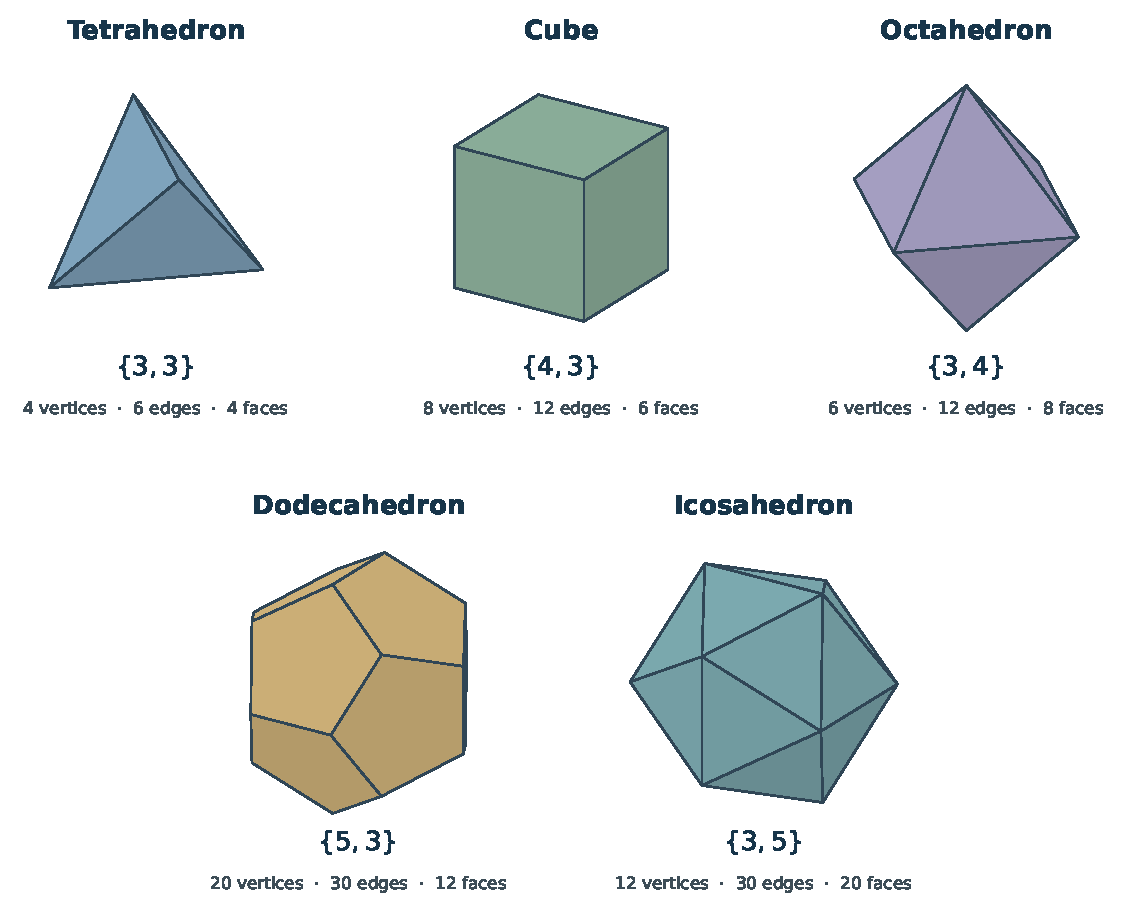
\includegraphics[width=0.97\linewidth]{platonic_models.pdf}
 \caption{The five exact coordinate constructions, rescaled separately
 to a common circumradius for this orthographic illustration.  The
 Schl\"afli symbol $\{p,q\}$ records $p$ edges per face and $q$ faces
 at each vertex.  The coordinates, facet lists and incidence counts
 are established algebraically in this section.}
 \label{fig:five-models}
\end{figure}

\subsection{A finite criterion for a complete facet list}

A facet of a three-dimensional finite convex hull contains three
affinely independent vertices and is the maximizing set of a nonzero
linear functional.  For the present coordinate sets, the normal can
always be chosen in $\Q(\varphi)^3$: take the cross product of two
differences of such facet vertices, and choose its supporting
orientation.  Consequently, all normal-sign cases below are decidable
algebraic cases.  They do not use trichotomy for arbitrary real numbers,
even when the resulting polytope is interpreted in $\R^3$.

This observation also gives a bounded verification procedure: examine
all vertex triples, discard collinear triples, and retain those planes
whose remaining vertices lie on one side.  However, the proof below
does not leave facet completeness to this procedure.  It explicitly
classifies the possible maximizing sets.

\subsection{Tetrahedron, cube and octahedron}

Write the four elements of $T$ as $v_0,v_1,v_2,v_3$.
Their squared norms are $3$, and $v_i\cdot v_j=-1$ for $i\ne j$.
The facet opposite $v_i$ therefore lies in
\[
 (-v_i)\cdot x=1;
\]
the other three vertices attain $1$, whereas $v_i$ gives $-3$.
The four vertices are affinely independent.  Every facet contains at
least three of them, so these four triangles are the complete facet list.
Every pair of distinct vertices has squared distance $8$; the faces are
congruent equilateral triangles.  Each vertex lies on exactly three
faces.  This constructs $\{3,3\}$ with $(V,E,F)=(4,6,4)$.

For $C$, a functional with normal $(a,b,c)$ is maximized by choosing the
sign of each vertex coordinate to agree with the corresponding nonzero
normal coordinate.  A vertex sign is free precisely where that normal
coordinate is zero.  A two-dimensional maximizing set therefore occurs
exactly when the normal has one nonzero coordinate.  The six facets are
\[
 x_i=1\quad\hbox{or}\quad x_i=-1\qquad(1\le i\le3).
\]
Each is a square of side $2$, and three meet at every vertex.
This constructs $\{4,3\}$ with $(V,E,F)=(8,12,6)$.

For $O$, the maximum of the same functional is
$\max(|a|,|b|,|c|)$.  To have three affinely independent maximizing
vertices, all three absolute values must be equal and nonzero.
Thus the eight facets have equations
\[
 s x_1+t x_2+u x_3=1,
 \qquad s,t,u\in\{-1,1\},
\]
and respective vertices $s e_1,t e_2,u e_3$.
Every such triangle is equilateral with squared side length $2$.
At a fixed vertex, one of the three signs is fixed and the other two
are free, so four faces meet there.  This constructs $\{3,4\}$ with
$(V,E,F)=(6,12,8)$.

\subsection{The icosahedron: twenty equilateral facets}

The set $I$ is invariant under independent coordinate sign changes and
cyclic coordinate permutations.  We can therefore take a supporting
normal to be $(a,b,c)$ with $a,b,c\ge0$.  If one coordinate is zero,
a cyclic permutation moves it to the first position.  The maximum of
this functional on $I$ is
\begin{equation}\label{eq:ico-maxima}
 \max(L_1,L_2,L_3),\qquad
 L_1=b+\varphi c,\quad
 L_2=a+\varphi b,\quad
 L_3=\varphi a+c.
\end{equation}

Suppose first that $a,b,c>0$.  Each $L_i$ corresponds to just one
candidate vertex.  A facet requires at least three maximizing vertices,
so $L_1=L_2=L_3$.  The first two equalities give
\[
 a=\varphi c-\psi b,
 \qquad \varphi b=\psi a+c.
\]
Substitution and $\varphi\psi=1$ give
\[
 (\varphi+\psi^2)b=2c.
\]
Since $\varphi+\psi^2=2$, we obtain $b=c$, and then $a=b$.
The facet normal is proportional to $(1,1,1)$.  Restoring signs gives
eight normals of the form $(\pm1,\pm1,\pm1)$.

Next suppose that $a=0$ and $b,c>0$.  Then
$L_3=c<L_1$.  The candidate for $L_1$ is $(0,1,\varphi)$, while
$L_2=\varphi b$ has two candidate vertices $(1,\varphi,0)$ and
$(-1,\varphi,0)$.  There are three maximizing vertices exactly when
\[
 b+\varphi c=\varphi b,
 \qquad\hbox{equivalently}\qquad b=\varphi^2 c.
\]
Its normal is proportional to $(0,\varphi,\psi)$.
Restoring signs and cyclic positions gives twelve more facet normals.
Finally, if two normal coordinates vanish, precisely two vertices
maximize the functional, so its maximizing set is an edge, not a facet.

We have proved that the complete list of supporting facet planes is
\begin{equation}\label{eq:ico-facets}
 n\cdot x=\varphi^2\qquad(n\in D).
\end{equation}
For $n=(1,1,1)$ the maximizing triangle is
\[
 (0,1,\varphi),\quad (1,\varphi,0),\quad (\varphi,0,1).
\]
For $n=(0,\varphi,\psi)$ it is
\[
 (0,1,\varphi),\quad (1,\varphi,0),\quad (-1,\varphi,0).
\]
These cover the two normal orbits under the displayed coordinate
symmetries.  The squared distances between adjacent listed points are
$4$, using
\[
 1+\psi^2+\varphi^2=4;
\]
the edge from $(1,\varphi,0)$ to $(-1,\varphi,0)$ visibly has squared
length $4$ as well.  Thus all twenty facets are congruent equilateral
triangles of side $2$.

The signed cyclic coordinate symmetries act transitively on the twelve
vertices of $I$.  At $(0,1,\varphi)$, the normals from
\eqref{eq:ico-facets} attaining equality are exactly
\[
 (1,1,1),\quad(-1,1,1),\quad(0,\varphi,\psi),\quad
 (\psi,0,\varphi),\quad(-\psi,0,\varphi).
\]
There are five, so every vertex has valence five.
Counting the three edges of every triangle, with each edge counted
twice, gives $2E=3\cdot20$ and hence $E=30$.
This constructs $\{3,5\}$ with $(V,E,F)=(12,30,20)$.

\subsection{The dodecahedron: twelve regular pentagonal facets}

The set $D$ has the same signed cyclic coordinate symmetries.
For a normal $(a,b,c)$ with $a,b,c\ge0$, the maximum on $D$ is
\begin{equation}\label{eq:dodeca-maxima}
 \max(M_0,M_1,M_2,M_3),
 \quad
 \begin{aligned}
 M_0&=a+b+c, & M_1&=\varphi b+\psi c,\\
 M_2&=\varphi a+\psi b, & M_3&=\psi a+\varphi c.
 \end{aligned}
\end{equation}

If $a,b,c>0$, each expression has a unique candidate vertex.
We show that three of them cannot maximize simultaneously.
If $M_0=M_1=M_2$, then
\[
 a=\psi b-\psi^2 c,
 \qquad c=\psi a-\psi^2 b.
\]
Substitution gives $c=-\psi^3c$, impossible because $c>0$.
Cyclic symmetry treats the other two choices involving $M_0$ and two
noncube candidates.  If instead $M_1=M_2=M_3\ge M_0$, their sum would
be at least $3M_0$.  But their actual sum is
\[
 (\varphi+\psi)(a+b+c)<3(a+b+c)=3M_0,
\]
again impossible.  Consequently no facet has an all-positive normal.

Let $a=0$ and $b,c>0$.  We have $M_2=\psi b<M_0$.
Set $t=b-\psi c$.  The two remaining comparisons are particularly
simple:
\[
 M_1-M_0=\psi t,\qquad M_0-M_3=t.
\]
If $t>0$, only $M_1$ maximizes and there is one maximizing vertex.
If $t<0$, only $M_3$ maximizes and the zero first coordinate of the
normal permits two maximizing vertices.
If $t=0$, the maximizing vertices are exactly
\begin{equation}\label{eq:pentagon-vertices}
 \begin{aligned}
 A&=(1,1,1), & B&=(0,\varphi,\psi), & C'&=(-1,1,1),\\
 D'&=(-\psi,0,\varphi), & E'&=(\psi,0,\varphi).
 \end{aligned}
\end{equation}
The normal is proportional to $(0,1,\varphi)$.
Restoring signs and cyclic positions gives twelve facet normals.
When two normal coordinates vanish, only two vertices maximize,
so this last case contributes no further facets.
The complete facet list is therefore
\begin{equation}\label{eq:dodeca-facets}
 n\cdot x=\varphi^2\qquad(n\in I).
\end{equation}

Here is an entirely algebraic verification that the five vertices in
\eqref{eq:pentagon-vertices} form a regular pentagon.
Let $(v_0,v_1,v_2,v_3,v_4)=(A,B,C',D',E')$, with indices taken modulo
five, and put $n=(0,1,\varphi)$.
Substitution in \eqref{eq:golden-identities} gives
\begin{align}
 \lVert v_{i+1}-v_i\rVert^2&=4\psi^2,
 &\lVert v_{i+2}-v_i\rVert^2&=4,
 \label{eq:pentagon-distances}\\
 n\cdot\bigl((v_{i+1}-v_i)\mathbin{\times}(v_{i+r}-v_i)\bigr)
 &=
 \begin{cases}
  6-2\varphi,&r=2,4,\\
  4\varphi-2,&r=3.
 \end{cases}
 \label{eq:pentagon-orientation}
\end{align}
For example,
\[
 \lVert B-A\rVert^2
 =1+\psi^2+\psi^4
 =8-4\varphi=4\psi^2,
 \qquad \lVert C'-A\rVert^2=4.
\]
All values in \eqref{eq:pentagon-orientation} are positive, so every
other vertex lies strictly on the same side of each oriented side
$v_iv_{i+1}$.  Thus the displayed order is the convex boundary order;
in particular it is not a star-polygon ordering.

By \eqref{eq:pentagon-distances}, cyclic shift preserves every pairwise
distance.  A distance-preserving assignment of three noncollinear
points extends uniquely to an isometry of their plane: subtract one
point, use its two independent difference vectors as a basis, and
compare their Gram matrices.  The distances to those three points then
determine every remaining point uniquely in the plane, so this isometry
sends each $v_i$ to $v_{i+1}$.
Its fifth power fixes three noncollinear points and hence is the
identity, while the isometry itself is nontrivial.
It preserves the centroid, has order five, and therefore is an
orientation-preserving plane rotation.  Together with the convex
boundary order, this proves that the facet is a regular pentagon.
This argument uses only finite dot products and nonzero determinants;
no trigonometric functions or limiting argument are required.

All normals in $I$ are carried to one another by the signed cyclic
coordinate symmetries, which preserve $D$.  Hence all twelve
pentagonal facets are congruent.
There are two vertex orbits to check for valence.  At $(1,1,1)$ the
incident facet normals are
\[
 (0,1,\varphi),\quad(1,\varphi,0),\quad(\varphi,0,1).
\]
At $(0,\varphi,\psi)$ they are
\[
 (0,1,\varphi),\quad(1,\varphi,0),\quad(-1,\varphi,0).
\]
The complete normal list \eqref{eq:dodeca-facets} shows that these
lists are exhaustive.  Thus precisely three faces meet at every
vertex.  Counting the five sides of the twelve facets gives
$2E=5\cdot12$, so $E=30$.
This constructs $\{5,3\}$ with $(V,E,F)=(20,30,12)$.

\subsection{Existence certificates and distinction of the five types}

For convenient reference, the exact metric data are collected below.
Here $\ell$ is the common edge length and $R$ the circumradius of the
coordinate model as written; the models have not been normalized to a
common edge length.
\begin{center}
\begin{tabular}{lcccc}
\hline
Solid & $\{p,q\}$ & $(V,E,F)$ & $\ell^2$ & $R^2$\\
\hline
Tetrahedron  & $\{3,3\}$ & $(4,6,4)$   & $8$ & $3$\\
Cube         & $\{4,3\}$ & $(8,12,6)$  & $4$ & $3$\\
Octahedron   & $\{3,4\}$ & $(6,12,8)$  & $2$ & $1$\\
Icosahedron  & $\{3,5\}$ & $(12,30,20)$ & $4$ & $\varphi+2$\\
Dodecahedron & $\{5,3\}$ & $(20,30,12)$ & $4\psi^2$ & $3$\\
\hline
\end{tabular}
\end{center}

Every item used in these constructions is finite and exact: coordinate
pairs in $\Q(\varphi)$, dot and cross products, supporting-plane
inequalities, face cycles and incidence lists.  The accompanying
\texttt{exact\_models.py} independently enumerates all supporting
vertex triples, verifies regular face Gram matrices and the complete
incidences, and exports the resulting finite data in
\texttt{certificates.json}.  It additionally checks exact orthogonal
symmetries acting transitively on all incident vertex--edge--face
flags.  These executable checks support the construction and supply
formalization data; the preceding human proof does not assume their
correctness, and their execution is not itself a kernel-checked proof
in $\ipra$.

\begin{proposition}\label{prop:five-examples}
All five pairs
$\{3,3\},\{4,3\},\{3,4\},\{3,5\},\{5,3\}$ have convex
Platonic realizations over $\Q(\varphi)$.  These five realizations are
pairwise nonsimilar.
\end{proposition}
\begin{proof}
The facet, regularity and valence verifications above prove existence.
A similarity preserves extreme vertices, whereas the five vertex counts
are the distinct numbers $4,8,6,12,20$.  No two displayed realizations
can therefore be similar.
\end{proof}

\section{Why the complete argument fits \texorpdfstring{$\ipra$}{iPRA}}\label{sec:internal}

We now assemble the proof of Theorem~\ref{thm:main}. This section also
specifies the distinction between a human proof of formalizability and
an already kernel-checked derivation.

\subsection{The returned witness and all search bounds}

Run the validator on the finite tower and polyhedron data. It parses
finite strings, evaluates the fixed scalar operations of Section~1,
and compares the finitely many incidence and metric entries. For an
invalid input, all output functions return fixed default values.
For a valid input, the following construction is total.
\begin{enumerate}
\item Form the edges and cyclic vertex links from the facet cycles.
Fan-triangulate the facets and try the explicitly bounded height
candidates. The lower-neighbor count proves Euler's identity.
\item Perform the two incidence counts and the natural-number
calculation~\eqref{eq:core}. Return the appropriate one of the five
type indices. The table proves $V\leq20$, $E\leq30$, $F\leq20$.
\item Use the finite reconstruction of Section~\ref{sec:maps}, or
enumerate at most $V!\leq20!$ vertex permutations, to match the face
incidences to the corresponding explicit model.
\item Scale to the common edge length and use the finite rigidity
argument. It proves that the corresponding complete vertex distance
matrices agree up to one positive factor. This is the existence
proof for a successful similarity test; it is not inferred just
from a numerical search failing to find a counterexample.
\item Extract an affine similarity by linear algebra. Choose four
affinely independent input vertices by at most $\binom V4$ tests.
If their images are $y_0,y_1,y_2,y_3$, set
\[
 U=[x_1-x_0\ \ x_2-x_0\ \ x_3-x_0],\qquad
 W=[y_1-y_0\ \ y_2-y_0\ \ y_3-y_0],
\]
\[
 A=WU^{-1},\qquad b=y_0-Ax_0.
\]
The proportional distance identities imply
$W^{\mathsf T}W=\lambda U^{\mathsf T}U$ and hence
$A^{\mathsf T}A=\lambda I$. Distances to the four independent
vertices fix every remaining point: subtract their squared-distance
equations to obtain a nonsingular system of three linear equations.
Thus $Ax_i+b=y_i$ for every vertex. Return $A,b,\lambda$ and the
permutation, and check their identities explicitly.
\end{enumerate}

The final step avoids requiring a separately stored square root of
the scale. All its entries use the common input field with $\sqrt5$
adjoined for the model. If permutations rather than the constructive
map reconstruction are used, choose the least permutation passing
this finite similarity test. The proof above guarantees that one
exists. Bounded least search is primitive recursive.

The auxiliary algorithms also have direct finite bounds. A spanning
tree is found by at most $V$ rounds of reachability; a permutation
cycle is followed for at most the number of its elements; supporting
planes require at most $\binom V3$ triples. The arm reduction shortens
its vertex list at each recursive step. Its event list has a finite
quadratic number of determinant constraints, each with at most two
roots, and the relevant lists here have at most seven vertices.
Finite minimum selection uses exact order. Arithmetic code sizes
are bounded by iterating~\eqref{eq:bitbound}. All these bounds are
primitive recursive functions of the input code.

\subsection{Quantifier-free induction, including the field-law issue}

Every list count, invariant check, permutation check, and finite
conjunction can be expressed as a Boolean primitive recursive
function. Induction on its prefix length is therefore induction
on an equation. Geometric language in the proof denotes determinant,
dot-product, incidence, and order conditions on such finite codes.
The rational and natural-number identities used in the local steps
are established from their defining equations by quantifier-free
induction.

There is a particular induction pitfall worth resolving explicitly.
One should not induct on the unbounded statement ``all field laws
hold for all elements of the first $j$ tower stages.'' Fix instead a
total height $N$, a final coefficient budget $H$, and the finite list
of local ordered-field proof templates in Lemma~\ref{lem:orderedstage}.
Let $K$ bound the number
of lower-stage operations in any one of these fixed templates, and set
\[
 F_N(B)=(B+2)2^{K L(N)},\qquad
 H_j=F_N^{\,N-j}(H).
\]
At stage $j$, take the primitive recursive Boolean conjunction of
the required law instances for all coefficient arrays within budget
$H_j$ in the fixed prefix tower. At stage $j+1$ every lower-stage
instance generated by a proof template lies within $H_j$. Finite
tuple enumeration and a prefix-fold induction establish the next
conjunction. The invariant itself is an equation, so this uses only
quantifier-free induction. At $j=N$ extract the desired instances
and then universally close the original free parameters. The
constant $K$ describes a fixed finite family of algebraic proofs;
it is not an interpreter for arbitrary proofs or programs.

The same bounded-table discipline applies when an induction appears
to range over all finite configurations of a given size: fix the
input and a primitive recursive bound on every configuration used
by its proof, and express the invariant as the corresponding finite
Boolean fold. No induction over arbitrary real predicates is
being smuggled into the argument. Formalizing the local templates
and their compatibility with represented equality is an explicit
obligation in the Lean plan.

We have now proved the classification assertion of
Theorem~\ref{thm:main}. Section~\ref{sec:existence} supplies five
valid fixed codes. They have distinct vertex counts, so a similarity
cannot identify any two of them. This proves the exact number five
inside the finite interpretation.

\section{Lean formalization: concrete interfaces and remaining work}
\label{sec:lean}

\subsection{Repository snapshot actually inspected}

The repository inspection is pinned to ProveIt commit
\begin{center}
\code{2811f73af20330d04bf3dae8428f87f7efa6580d}.
\end{center}
Its toolchain specifies Lean \code{v4.32.0} and Mathlib
\code{v4.32.0}. The following interfaces already exist in the
\code{ConciseIPRA} library~\cite{proveit}:
\begin{center}
\begin{tabular}{p{0.30\linewidth}p{0.60\linewidth}}
\toprule
Interface & Purpose\\
\midrule
\code{PR k}, \code{PTm n} & Primitive recursive symbols and terms.\\
\code{PRAAx} & Defining equations, successor axioms, and quantifier-free induction.\\
\code{Prf PRAAx} & Deeply embedded intuitionistic derivability.\\
\code{PRA.qfInd} & Derived interface for quantifier-free induction.\\
\code{NFm.ofPRA} & Translation into the native scalar syntax.\\
\code{pra\_iff\_native} & Transport of a completed internal arithmetic derivation.\\
\bottomrule
\end{tabular}
\end{center}
The supplied \code{docs/drafts} directory was inspected for relevant
material. Its binary draft archives are not assumed as proved
dependencies. The argument here is self-contained at the level of
ordinary human-readable mathematical proof.

\subsection{What the supplied Lean source does}

The standalone file \code{lean/Arithmetic.lean} supplies candidate
proof terms, through tactics, for the numerical middle of the argument:
\begin{itemize}
\item $p,q\geq3$ and $pq<2p+2q$ imply one of the five ordered pairs;
\item the incidence equations and Euler identity imply that inequality;
\item the five full $(p,q,V,E,F)$ rows follow;
\item the explicit candidate-pair list has length five and no repetitions.
\end{itemize}
These are ambient Lean theorems about integers, conditional on the
stated counting hypotheses. They do not assert that Euler or geometric
rigidity has already been formalized. The file has no proof holes or
new axiom declarations, but \textbf{it has not been compiled}: Lean,
Lake, and Elan were unavailable in the production environment.
It is implementation material to build and review, not a claimed
kernel-checked result.

The adapter \code{lean/ConciseBridge.lean} demonstrates the exact
last transport. In mathematical Lean notation its interface is
\begin{verbatim}
(phi : Fm PTm 0) ->
Prf PRAAx [] phi ->
NPrf [] (NFm.ofPRA phi).
\end{verbatim}
Its derivation argument is an explicit premise. The adapter does not
pretend to supply the missing internal classification proof.

\subsection{A dependency-ordered completion plan}

The following modules give a direct route to a full formalization.
The rightmost column states an actual proof obligation, rather than
merely naming a large theorem to import.
\begin{longtable}{p{0.20\linewidth}p{0.70\linewidth}}
\toprule
Module & Required result\\
\midrule
\endhead
\code{Coding} & PR list, array, signed-rational, and bounded-fold operations;
equational induction lemmas and explicit register bounds.\\
\code{Radicals} & The sign and inverse algorithms, redundant-stage equality,
operation compatibility, and the bounded-table proof of ordered-field laws.\\
\code{FinitePolyhedron} & PR support-triple enumeration, exact regular-face
and incidence checks, and correctness of the finite hull representation.\\
\code{EulerSweep} & Generic-height search, convex vertex-figure block lemma,
and the accumulator proof $V+F=E+2$.\\
\code{FivePairs} & An actual \code{Prf PRAAx} derivation of
$Eab+2pq=4E$ and the five-way disjunction. Ambient \code{omega} is not
a replacement for this embedded derivation.\\
\code{FiveMaps} & The tetrahedral and octahedral graph arguments, Schlegel
triangle test, disk count, twelve-vertex reconstruction, and finite duality.\\
\code{FiniteRigidity} & The algebraic hinge and triangle comparisons,
quadratic event list, arm reduction, sign changes, rotation-cycle deletion,
and face propagation. The relevant arm sizes can be unrolled.\\
\code{Models} & The five exact coordinate tables and successful evaluations
of the support, regularity, and incidence validators, with their correctness
theorems.\\
\code{Classification} & Total PR classifier and similarity witness;
the internal closed classification formula; transport by
\code{pra\_iff\_native}.\\
\bottomrule
\end{longtable}

The final central theorem must have the type
\begin{verbatim}
Prf PRAAx [] classificationFormula
\end{verbatim}
where \code{classificationFormula : Fm PTm 0} encodes
Theorem~\ref{thm:main}. Proving a theorem about \code{Real}, obtaining
a successful Python run, or even proving the complete theorem in
ambient Lean would not alone establish this type. A completed build
should also retain \code{\#print axioms} output for the final derivation
and record the exact repository revision.

\section{Artifact and verification record}\label{sec:artifacts}

\subsection{Exact executable certificate}

The Python program \code{code/exact\_models.py} uses rational pairs
$a+b\varphi$, where $\varphi^2=\varphi+1$. It uses no floating point,
symbolic algebra system, or numerical convex-hull library. It
enumerates supporting triples and checks the complete facet list,
convex cyclic order, face Gram matrices, congruence, edge incidences,
connected cyclic vertex links, and the numerical identities.

As an additional check, it enumerates the orthogonal maps obtained
by sending a fixed vertex basis to every ordered triple with the
same Gram matrix. Every resulting matrix is checked against every
vertex. It finds respectively $24,48,48,120,120$ symmetries and
verifies transitivity on all vertex-edge-face flags. This stronger
symmetry property is verified for the examples; it was not assumed
in the classification input.

All five model verifications passed. The largest model has twenty
vertices, giving $\binom{20}{3}=1140$ unordered supporting triples
and $20\cdot19\cdot18=6840$ ordered basis-image triples. The JSON
certificate stores the exact vertices, ordered facets, support planes,
edges, incidences, and symmetry matrices. Each pair of strings
\code{["a","b"]} denotes $a+b\varphi$ with rational $a,b$.
The figure renderer uses floating point only to draw these already
certified coordinate lists; it is not part of the proof verifier.

\subsection{Status table}

\begin{center}
\begin{tabular}{>{\raggedright\arraybackslash}p{0.43\linewidth}>{\raggedright\arraybackslash}p{0.47\linewidth}}
\toprule
Deliverable & Status\\
\midrule
Human classification and $\ipra$ interpretation & Complete argument in this article.\\
Five exact models and finite certificates & Executed successfully; reproducible Python log included.\\
LaTeX article and PDF & Compiled and visually checked before delivery.\\
Ambient Lean arithmetic prototype & Source reviewed; uncompiled in this environment.\\
Full embedded geometric \code{Prf PRAAx} derivation & Not completed; precise modules and proof obligations listed above.\\
\bottomrule
\end{tabular}
\end{center}

\clearpage
\begin{thebibliography}{9}
\raggedright
\bibitem{euclid}
Euclid, \emph{Elements}, Book XIII, constructions in Propositions 13--17
and classification remark following Proposition 18.
Clay Mathematics Institute historical edition,
\url{https://www.claymath.org/library/historical/euclid/files/elem.13.18.html}.

\bibitem{sz}
I. J. Schoenberg and S. K. Zaremba,
\emph{On Cauchy's lemma concerning convex polygons},
Canadian Journal of Mathematics \textbf{19} (1967), 1062--1071.
Corrected short induction: Section 3, pp.\ 1070--1071.
\url{https://doi.org/10.4153/CJM-1967-096-4}.

\bibitem{bowers}
J. C. Bowers, P. L. Bowers, and K. Pratt,
\emph{Cauchy rigidity of c-polyhedra}, preprint, April 3, 2017,
Section 2 (review of classical Cauchy rigidity).
\url{https://www.math.fsu.edu/~aluffi/archive/paper518.old.pdf}.

\bibitem{proveit}
V. Reshetnikov and contributors, \emph{ProveIt},
\path{Logic/PrimitiveRecursiveArithmetic/ConciseIPRA},
snapshot \code{2811f73af20330d04bf3dae8428f87f7efa6580d}.
Files inspected include \code{PR.lean}, \code{Deduction.lean},
\code{NativeBiInterpretation.lean}, and the directory README.
\url{https://github.com/VladimirReshetnikov/ProveIt/tree/2811f73af20330d04bf3dae8428f87f7efa6580d/Logic/PrimitiveRecursiveArithmetic/ConciseIPRA}.

\bibitem{wiki}
\emph{Platonic solid}, Wikipedia, the reference specified in the task,
consulted November 15, 2026. Used to fix the usual local definition and
classical target; the arguments in this article supply the proof.
\url{https://en.wikipedia.org/wiki/Platonic_solid}.
\end{thebibliography}
\end{document}
